\section{Introduction}
%% {\bf [ID/Locator split is the way to solve 4 issues in current
%% Internet including routing scalability, mobility support,
%% multi-homing
%% support and traffic engineering enhancements]}
The concept of separating identifiers from routable addresses or locators has been advocated by a number of authors in the networking community~\cite{saltzer,bennett,moskowitz,milsa}.
%There is a long history in the networking community separating the binding between identifier names and addresses -- the network-attached object named in the communication is separate from the network structure.That is, the sources and destinations should not be implicitly or explicitly bound to the network topology.
Separation of names from addresses makes it possible to avoid implicit or explicit binding of sources and destinations to the network's actual topology. 
Using existing terminology, the {\em identifier} names a
communicating object, such as a particular mobile phone, while the {\em locator}
identifies an address the network can use to route messages. For example,
a phone connecting to different 3G, 4G, and WiFi networks would get a separate
locator for each network. However, the identifier,
which in this case could be the International Mobile Subscriber Identity (IMSI) number, would remain the same. The goal of this work is to explore the
feasibility of identifier based communication under the assumption of large-scale dynamic mobility of named objects. In the above example, programmers should be able to send messages to a particular phone based on its IMSI number rather than to
an IP address. We take the position that identifiers can also be used to name
abstract entities and services; they need not to be tied to a particular
device. %However, the identifier should not be bound to any particular
%network topology.

%%{\em \bf why are global IDs good?}
Identifier based communication has many advantages, including simplified implementation session management, multi-homing, mobility, disconnection, authentication and
security~\cite{saltzer,bennett,moskowitz,milsa}.
When there is a high degree of dynamism between the communicating entities
and the network (as in most mobile service, content retrieval and cloud computing scenarios), using identifiers  to define network-attached objects is more appropriate than using locators.
Intuitively, it is easier to work with networking primitives based on identifiers when the locator changes faster than the
timescales of the communication session. For example, a voice call may last 30 minutes,
but a mobile device in a vehicle may change its network attachment points
many times during this period.

%%Requiring application developers to manage
%%variable and missing locators places an
%%undue burden on them compared to
%%expressing identity and then having the network manage the locators.
%%In addition, expressing identity allows the re-use of
%%the management software across many applications.
%%Finally, expressing identifiers allows the possibility of the
%%network using them for routing, buffering and authentication as well.

%%{\em \bf what we are doing an why it is hard about this:}

%%In this work we seek enabling technologies toward practical
%%implementation communications using global identifiers instead of
%%the current locator based approach, i.e., all
%% receiving messages based on global IDs rather than IP addresses.
Realizing an identifier based protocol stack has
several challenging aspects; the key design issue we address in this work is the
dynamic binding of identifiers to locators. That is, when the user presents
the networking stack with an identifier, the networking subsystem
must quickly return a set of locators, or {\em network addresses} (NAs)
back to the user. We address the challenge of providing a fast global name resolution service at Internet scale in this paper, and describe and evaluate a specific \textit{Direct Mapping (\textbf{DMap})} scheme for achieving a good balance between scalability, low update/query latency, consistency, availability and incremental deployment.

We take note of two trends in the Internet community that have significant bearing on the design of a global name resolution scheme. First, a flat identifier space is preferred to the hierarchical domain names currently used in the Internet. The use of flat, location independent identifiers is a central tenet of a number of clean slate proposals such as AIP~\cite{andersen}, HIP~\cite{moskowitz}, ROFL~\cite{CaesarRofl} and MobilityFirst~\cite{mobilityFirst}. The key advantage of flat labels lies in their use for direct verification of the binding between the name and an associated object (see~\cite{Ghodsi-ICN} for a detailed discussion).  As a result, name resolution schemes that rely on the hierarchical structure of the name such as the Domain Name System (DNS) or LISP-TREE~\cite{jakab} are not suitable for supporting such a flat identifier space.

The second trend is that due to its separation from the network attachment point, global names or identifiers will tend to belong to end-users or application providers rather than to the network, as is currently the case with IP. Hosts and other network-attached objects (content, computing services, etc.) are not owned by any Internet Service Provider (ISP), but they just happen to be connected to a particular Autonomous System (AS). Most name resolution schemes propose to store the mappings of the identifiers belonging to an AS inside that AS only~\cite{mathy}. The same rationale, however, does not work for a host-based identifier space because hosts (or content) do not belong to any particular AS, especially with the increasing number of mobile hosts which often have multiple simultaneous points of network attachment. Thus we challenge the assumed constraint of ownership based storage and design a scheme with network-wide sharing of the identifier-locator mappings independent of the AS boundaries.
 \begin{center}
        %\vspace{-0.2in}
        \begin{figure}[t]
            \centering           
            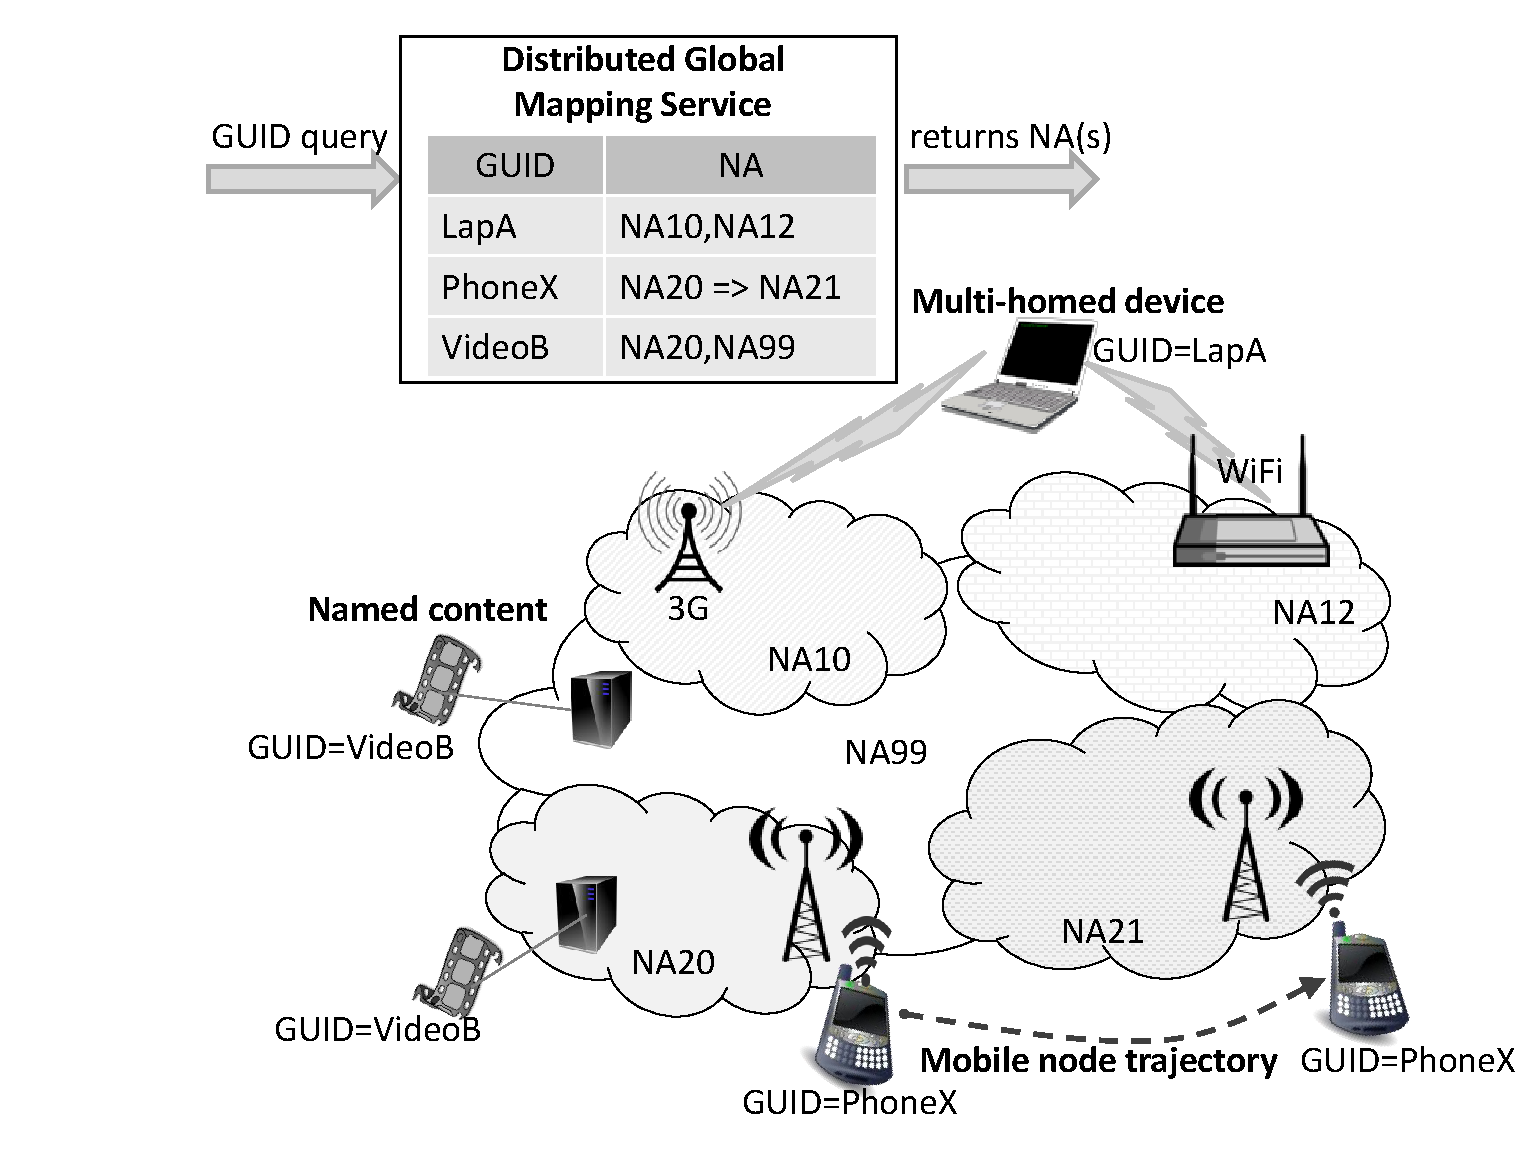
\includegraphics[ trim = 0.1in 0in 0in  0.1in, clip,width=0.5\textwidth]{figures/overview.eps}
            \vspace{-0.1in}
            \caption{Distributed global identifier to locator mapping service}
            \label{fig:overview}
			\vspace{-0.15in}
        \end{figure}

    \end{center} 
\vspace{-0.3in} 
% \hspace{0.1in}

Motivated by these trends, we propose a dynamic identifier to locator mapping management scheme called DMap which supports a flat space of a identifiers, referred to as {\em Globally Unique Identifiers}, or GUIDs. A GUID is a long bit sequence, such as a public key, that is globally unique and long enough that the chance of a collision is infinitesimally small. Each end host, such as laptops, mobile phones, servers and virtual machines can have a GUID. In addition, even abstract objects, such as a piece of content or a particular context, can have GUIDs. Each GUID is associated with one or more network addresses (NAs) that it attaches or belongs to. For example, the NAs of a multi-homed laptop in Figure~\ref{fig:overview} includes the NA of its 3G service provider and the NA of the network that its WiFi interface attaches to. We denote the identifier to locator mapping as the GUID$\rightarrow$NA mapping.

To perform the mapping service for a given GUID, DMap applies $K (K>1)$ hashing functions onto it to produce a list of $K$ network addresses, which are IP addresses in today's Internet, and stores the GUID$\rightarrow$NA mapping in the ASs that announce those network addresses. By doing so, DMap spreads the GUID$\rightarrow$NA mappings amongst ASs, such that an AS will host mappings of other ASs, as well as have its mappings hosted by others. A key advantage of this {\em shared hosting} approach is that it allows the hosting ASs to be deterministically and locally derived from the identifier by any network entity. DMap is simple yet efficient. It leverages the routing infrastructure to reach the hosting AS in a single overlay hop; it does not require a home agent, unlike mobile IP and existing cellular networks. Further, the potential shortcoming of the direct mapping scheme, lack of locality, is addressed by having multiple copies of the mappings that are stored in multiple locations. We further improve the design by including a local copy of the mapping within the AS that the GUID is residing in (this AS may change as the host moves).

Through detailed simulation studies, we show DMap achieves a $95^{th}$ percentile round trip query response time of below 100ms, which is important to support the fast growing class of mobile devices connected to the Internet.
%
%
%We set as a target the ability to
%support voice application under these conditions,
%with frequent handoffs. 
%Existing cellular telecommunication networks typically support handoffs within 100-200 ms~\cite{3gpp}. 
Our results also show that DMap can proportionally distribute GUID$\rightarrow$NA mappings among ASs, which is critical to scale our system to support billions of GUIDs and NAs associated with a global scale network. 
%
%shares the scalability goals of many other works, in that
%it should scale to billions of GUIDs and NAs. If we wish to use GUIDs
%as a replacement for mobile phone applications, we need to support
%this level of scale. 
%DMap's approach to scale is to leverage
%the number and sizes of the participating ASs.
%
%We found DMap can support such
%low latencies by showing it can update the GUID to locator mapping,
%e.g., GUID$\rightarrow$NA,
%in this regime. Using DMap for these applications also means that any
%inconsistencies can be resolve in sub-second timescales.


%%{\em \bf why our approach is novel, and our contributions}

%Our approach, called direct mapping (DMAP), is unique in several ways.
%First, rather than a completely new design, we seek to
%enable incremental deployment by leveraging the
%existing Internet routing framework as much as possible.
%Our approach builds on top of the routing tables created by
%the Border Gateway Protocol (BGP). The existing routing tables
%give us a partial view that greatly simplifies the design.

%Second, DMAP assumes a different fairness and trust model compared to
%previous works. In many identifier based approaches, each
%Autonomous System (AS) ownes a set of identifiers, and stores mappings
%between identifiers and locators for its identifier set.


%DMAP also introduces a new fairness metric. In many schemes, each
%hosting entity is considered equal. However, in DMAP's approach,
%each entity, in our case an AS, should host a number of mappings
%proportional to the amount of network address space they claim. That is,
%a large Internet Service Provider (ISP), with many ASes and claiming
%a lot of IP address space must host many more mappings than
%a small ISP with a small amount of address space. This is intuitively
%fair because large ISPs claiming large fractions of the IP address space
%should also have a large number of customers, and thus a large
%number of mappings.

%We found that shared hosting leads to drastically reduced mapping resolution
%latency compared to Distributed Hash Table (DHT)
%based schemes without requiring any Domain
%Name System (DNS) like infrastructure services. In addition, it allows us
%to use a flat identifier space. Unlike other hierarchical based global name
%spaces, such as DNS, DMAP supports a flat space of a identifiers, that is,
%identifiers with no internal hierarchical structure. We call these
%{\em Globally Unique Identifiers}, or GUIDs. A GUID is a long bit sequence,
%such as a public key, that is globally unique and long enough that the chance
%of an accidental collision is infinitesimally small.




%That is, the 100,000's of ASs should support several

%We evaluate DMap using a trace driven simulation approach.
%Using existing popularity models, we first simulate a binding service
%workload. We then evaluate the query latency given the
%real AS graph, considering actual hop counts and latency distributions.
%We demonstrate that DMap's shared hosting approach is feasible and gives
%good performance, under 100 ms latency in most cases. We show that
%DMap is robust to BGP churn and router failures. Finally, we present
%an analytic model that evaluates the expected AS hop-count and latency needed
%to perform the mappings. The analytic results are in agreement with
%the simulation results. The model shows that
%current trends in the Internet would lead to further improvements in DMap's performance.

The rest of paper is organized as follows. In Section~\ref{sec:overview}, we provide the background and motivation for DMap. The working of DMap and how DMap addresses several technical challenges are discussed in Section~\ref{sec:design}. We present detailed simulation evaluation results in Section~\ref{sec:evaluation}, and an analytical model in Section~\ref{sec:model}. Finally, we have the related work in Section~\ref{sec:related} and the concluding remarks in Section~\ref{sec:conclusion}.


%% {\bf Simple figure capturing use case of GNRS inserted here}

%\subsection{Key Contributions}

%The main contributions that we make in this paper are:

%Based on these requirements we introduce a mapping distribution scheme in which, instead of each AS storing and managing its set of identifier-locator tables, each mapping entry is managed by a set of foreign ASs. We explain the reasons behind this choice, point out its benefits and address the evident incentive and privacy issues. Specifically, our approach leverages the locator reachability information (IP reachability in the present Internet context) that is readily available at the network layer, and makes use of an in-network single hop hashing technique to reach the storage point for any given identifier-locator mapping entry with low latency. We make the following key contributions in this paper:

%\begin{enumerate}
%\item
%We propose a co-operative identifier to locator mapping scheme that
%distributes the mapping entries among participating ASs without regard
%to ownership and AS boundaries. We enumerate its benefits and address
%the evident problems associated.
%We propose a conceptual shift from ASs `owning' endpoint identifiers and individually storing the mappings of its owned set of identifiers to a network-wide sharing of the identifier-locator mappings irrespective of the AS boundaries. Our scheme results in a natural order of incentives in which an AS which is expected to produce a large number of identifier-locator lookups from other ASs, itself stores and answers a proportionally large number of mappings. We aim to provide reasonings that show the feasibility of the scheme in order to open further research into this line of thought.

%\item
%We introduce a novel single-hop hashing technique in
%Section~\ref{sec:design} that leverages the IP reachability
%information available at the network layer for low-latency mapping
%queries. To lookup a mapping in this scheme, one can directly hash the
%identifier to produce the network address of the AS that stores its
%mapping.

%\item
%We validate our scheme through a large-scale discrete event simulation
%based on Internet measurement traces. We show in
%Section~\ref{sec:evaluation} that this scheme achieves low latency
%values with a 95th percentile value of $\sim$100 ms, a 2x - 5x
%reduction compared to previously published results.

%\end{enumerate}


%% vassiliou_2009, 802.11 latencies of 200-400 ms
%% Mishra:2003:EAI:956981.956990, mean latencies of 3-4 seconds

